% первая глава

\section{Формирование и планирование семейного бюджета}

\subsection{Семейный бюджет с точки зрения экономики}

Бюджет в переводе с английского означает роспись денежных доходов и
расходов на определенный срок. Применительно к семейной экономике главный смысл бюджета заключается в не превышении расходов над доходами
за определенный промежуток времени при условии удовлетворения необходимых потребностей.
Количественный бюджет семьи определяет ряд факторов: численность
семьи, наличие в ней работающих; пенсионеров, стипендиатов и иждивенцев; размер заработной платы; величина пенсий, стипендий, пособий; наличие личного транспорта, подсобного хозяйства, проживание в городской или
сельской местности; национальные особенности.
Для того чтобы эффективно использовать свои доходы, семья должна правильно составить свой бюджет, тщательно продумать покупки и делать сбережения для достижения своих целей. Для составления семейного бюджета
необходимо подготовить список всех источников доходов каждого члена семьи. Это зарплата, социальные пособия и проценты на сбережения. В статье
расходов нужно перечислить все, за что надо заплатить в течение месяца:
квартплата и услуги, питание, проезд, уплата налогов и взносов. В планируемые расходы так же включаются и сбережения на будущее.
Если доходы равны расходам, то это сбалансированный бюджет. Если
предполагаемые расходы превышают доходы, то этот бюджет имеет дефицит. Бюджет, в котором доходы превышают расходы, будет иметь избыток.
Если расходы превышают доход, необходимо исключить из планов лишние
покупки, чтобы сбалансировать бюджет.

\subsection{Источники доходов и статьи расходов}

\subsubsection{Доходы}

\textbf{Cемья} - это объединение людей, которое основано на браке или кровном родстве и связано общим бытом, семейными доходами и взаимной ответственностью.

\textbf{Семейный доход} - это денежные средства, которые члены семьи получают
от посторонних лиц или организаций и могут использовать для оплаты собственных расходов. Все семейные доходы подразделяются на 2 вида:
денежные и натуральные. Основными денежными доходами семьи обычно
являются следующие 4 группы доходов:
\begin{enumerate}
\item Оплата труда членов семьи (заработная плата);
\item Поступление из общественных фондов потребления (часть доходов семья получает в виде бесплатных услуг, денежных выплат, льгот);
\item Прочие (случайные) доходы (вознаграждения, наследство, подарки);
\item Доходы от домохозяйственной и предпринимательской деятельности.
\end{enumerate}
Натуральные доходы семьи могут быть в виде различной продукции собственного домохозяйства, готовой продукции предприятий выдаваемой ими
в счёт заработной платы, а также различные материально-вещественные ценности, получаемые членами семьи в порядке пособия, пожертвования, дарения и т.п. Натуральные доходы при их суммировании с денежными доходами
оцениваются по средним рыночным ценам в данном регионе на дату получения этих натуральных доходов.
Все суммированные денежные и натуральные доходы подразделяются на
несколько видов в зависимости от степени полноты их исчисления. Наиболее
полными являются совокупные доходы семьи, представляющие собой сумму всех денежных и натуральных доходов всех членов семьи. Все денежные
и натуральные доходы семьи, которые подлежат налогообложению, называются совокупными налогооблагаемыми доходами. А совокупные доходы за
вычетом всех налогов и обязательных платежей составляют располагаемые
или чистые доходы, поступающие в полное распоряжение семьи.

\subsubsection{Расходы}
Семейные расходы можно разделить на 4 группы:
\begin{enumerate}
\item Обязательные (жилищно-коммунальные услуги, телефон, медикаменты,
налоги);
Эта группа расходов имеет неприятное свойство - накапливаться в виде
долга, если они не производятся своевременно.
\item Текущие (продукты питания, транспорт, промышленные товары);
\item Периодические (досуг, развлечения); Эти расходы особенны тем, что носят вероятностный характер. Они могут быть в определ нном месяце, квартале, но могут и не появиться,
\item Единовременные расходы (приобретение значительных по стоимости вещей).
Производятся несколько раз в несколько лет.
\end{enumerate}

Кроме того, в течение года могут быть и одноразовые затраты - взносы в
общественные фонды, сезонные закупки, подписка, оплата пут вок в санаторий и т. п.
Так же в условиях продолжительных периодов анализа формирования семейного бюджета, нельзя не учитывать влияние на экономику семей столь
мощного процесса, как инфляция.

\subsection{Составление плана доходов и расходов семьи}
Для обеспечения стабильного материального положения семьи, а тем более для повышения ее благосостояния необходимо планирование семейного
бюджета.
Первой предпосылкой и обязательным условием планирования семейного
бюджета является учет доходов и расходов семьи.
Планирование семейного бюджета - это прогнозирование изменений доходов и расходов семьи на предстоящий период, определение организационноэкономических и финансовых мер по сбалансированности доходов и расходов,
получению и эффективному использованию семейных накоплений.
Планирование семейного бюджета осуществляется в следующем порядке:
\begin{enumerate}
\item Прогнозирование доходов семьи;
\item Прогнозирование расходов семьи;
\item Сопоставление предстоящих доходов и расходов;
То есть их балансировка и регулирование посредством поиска дополнительных источников доходов и определения мер по сокращению расходов семьи.
\item определение и распределение ожидаемых семейных накоплений.
\end{enumerate}
\pagebreak
Чтобы составить проект бюджета семьи, нужно ответить на три вопроса:
\begin{enumerate}
\item Сколько денег имеем;
\item Как их истратить, чтобы удовлетворить насущные потребности не влезая в долги;
\item Как распределить покупки во времени, увязав их с доходами и возможностями,предоставляемыми торговлей и предприятиями службы быта.
\end{enumerate}
ак и в экономике промышленных предприятий, в семейной экономике
должно быть годовое, месячное и недельно-суточное планирование. Исходным моментом составления бюджета семьи является оценка по доходной части во времени - на месяц, на год. Это заработная плата членов семьи плюс
выплаты из общественных фондов потребления. Желательно оценить возможные изменения составных частей дохода в планируемом периоде. Например, премиальные доплаты могут изменяться помесячно, поквартально, и их
при годовом планировании следует включать в расчет на среднем уровне по
прошлым периодам. Нужно оценить изменения в заработной плате в связи с возможностями повышения квалификации, повышением в должностной
иерархии или смену работы, которая приведет либо к прибавке, либо к уменьшению доходов. Также нужно учесть и возможное снижение доходов семьи
(например, переход одного из членов семьи на пенсию, рождение ребенка и
т. д.).
Доходы целесообразно учитывать ежемесячно, а сезонные (например, доходы от подсобного хозяйства) или единовременные - в расчете на квартал,
полугодие, год.
\begin{table}[H]
\caption{Пример таблицы}
\label{tab:t1}
\begin{center}
\begin{tabular}{|r|p{5.5cm}|p{2.5cm}|}
\hline 
1 & Первый текст в ячейке фиксированной ширины & $E=mc^2 $ \\ 
\hline 
12 & Второй текст тоже может быть произвольно длинным & $\sin \pi = 0 $ \\ 
\hline 
\end{tabular} 
\end{center}
\end{table}

\subsection{Вставка изображения}

\begin{figure}[H]
	\centering
	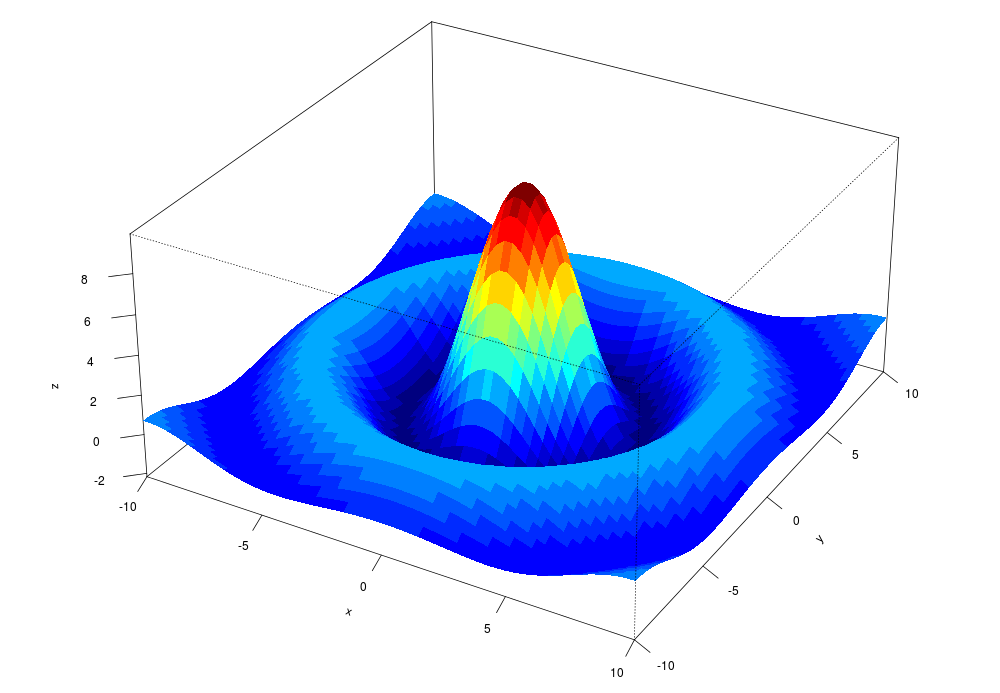
\includegraphics[width=0.7\linewidth]{pics/pic3D.png}
	\caption{Пример изображения для демонстрации возможности вставки в документ}
	\label{fig:pic3d}
\end{figure}



Изображение на рис.~\ref{fig:pic3d} находится в подкаталоге pics.

